\documentclass[12pt, twoside]{article}
\usepackage[letterpaper, margin=1in, headsep=0.5in]{geometry}
\usepackage[english]{babel}
\usepackage[utf8]{inputenc}
\usepackage{amsmath}
\usepackage{amsfonts}
\usepackage{amssymb}
\usepackage{tikz}
%\usetikzlibrary{quotes, angles}

\usepackage{graphicx}
\usepackage{enumitem}
\usepackage{multicol}

\usepackage{fancyhdr}
\pagestyle{fancy}
\fancyhf{}
\renewcommand{\headrulewidth}{0pt} % disable the underline of the header

\usepackage{setspace}
%\linespread{1.75}

%\fancyhead[RE]{\thepage}
\fancyhead[R]{\thepage \\ Name: \hspace{3cm}}
\fancyhead[L]{BECA / Dr. Huson / 12.1 IB Math SL\\* 19 March 2019}

\begin{document}
\subsubsection*{Do Now Quiz: Calculus \& Trigonometry - with calculator}
Pick one problem from each page.
 \begin{enumerate}

%\subsubsection*{You may use a calculator on these problems \hfill [34 marks]}

\setstretch{1.5}

\item \emph{Medium} Let $f(x)=6-x^2$. Part of the graph of $f$ is shown in the following diagram.
    \begin{center}
      \begin{tikzpicture}[xscale=1,yscale=0.7]
        \draw [thick, ->] (-3,0) -- (3,0) node [below] {$x$};
        \draw [thick, ->] (0,-2) -- (0,6) node [left] {$y$};
        \draw[thick, domain=-2.5:2.5] plot[samples=100](\x, {5-(\x)^2});
        \fill (-5^0.5, 0) circle[radius=0.05] node[above left]{$A$};
        \fill (5^0.5, 0) circle[radius=0.05] node[above right]{$B$};
      \end{tikzpicture}
    \end{center}
  \begin{enumerate}
    \item The graph crosses the $x$-axis at the points $A$ and $B$.\\
    Find the $x$-coordinate of $A$ and of $B$. \hfill [3]
    \item Find the area of the region enclosed by the graph of $f$ and the $x$-axis.  \hfill [3]
  \end{enumerate}

\item \emph{Spicy} The graph of $y=(x-1)\sin x$, for $0 \leq x \leq \frac{5 \pi}{2}$, is shown below.
      \begin{center}
        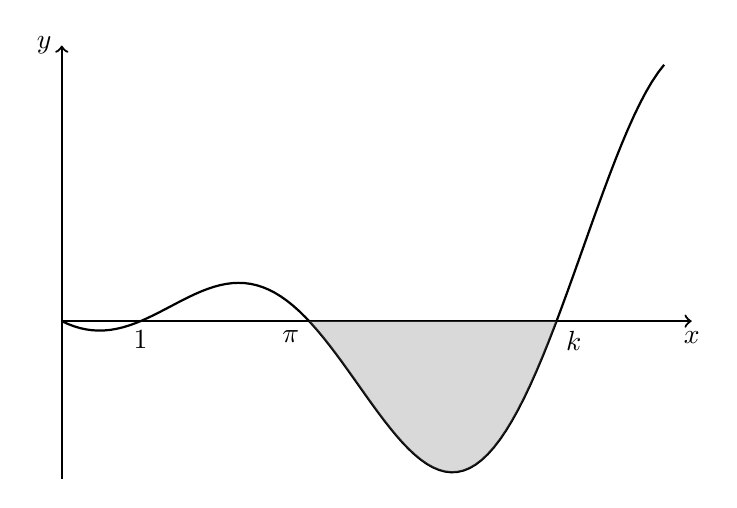
\begin{tikzpicture}[xscale=1,yscale=0.5]
          \draw [thick, ->] (0,0) -- (8,0) node [below] {$x$};
          \draw [thick, ->] (0,-4) -- (0,7) node [left] {$y$};
          \draw[thick, domain=0:7.65] plot[samples=100](\x, {(\x-1)*sin(\x r)});
          \draw (1, 0)node[below]{$1$};
          \draw (3.14, 0)node[below left]{$\pi$};
          \draw (6.28, 0)node[below right]{$k$};
          \fill[gray,opacity=.3] plot[domain=3.1416:6.283](\x, {(\x-1)*sin(\x r)});
          %\draw (1.5,1) node {$\mathbf{R}$};
        \end{tikzpicture}
      \end{center}
      \begin{enumerate}
        \item The graph has $x$-intercepts at $0,1, j, \text{ and }k$.
          Find $j$ and $k$. \hfill [2]
        \item The shaded region is rotated $360^\circ$ about the $x$-axis. Let $V$ be the volume of the solid formed. %\\
        Write down an expression for $V$. \hfill [3]
        \item Find $V$.  \hfill [2]
        \end{enumerate}

\newpage
\item \emph{Medium} Let $f(x)=3 \sin (\pi x)$.
  \begin{enumerate}
    \item Write down the amplitude of $f$. \hfill [1]
    \item Find the period of $f$. \hfill [2]
    \item On the following grid, sketch the graph of $y= f(x)$, for $0 \leq x \leq 3$.\\
    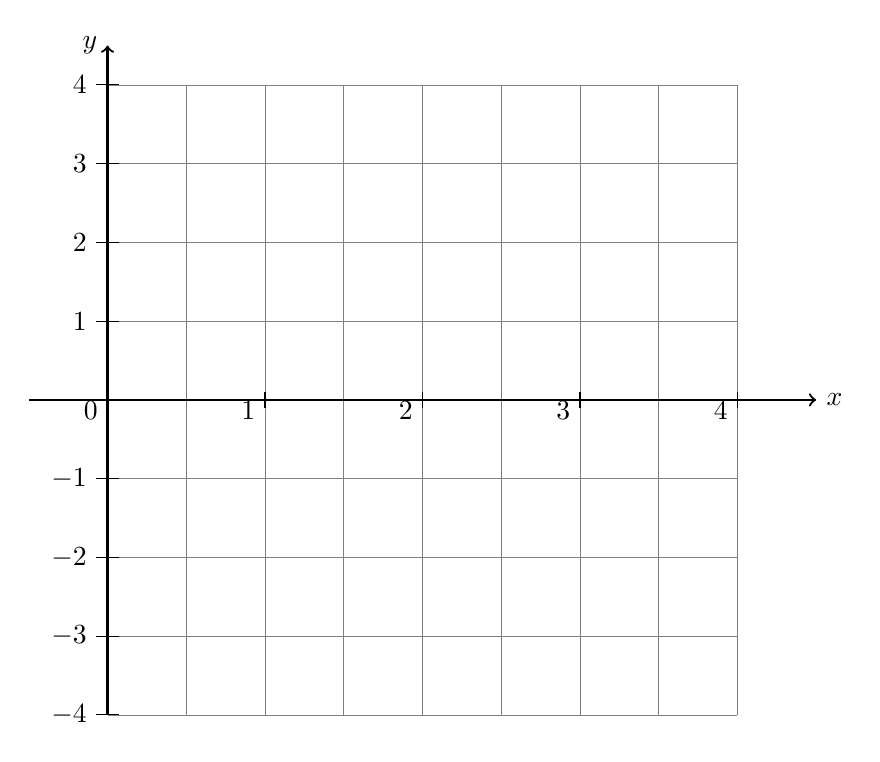
\begin{tikzpicture}[xscale=2.0]
      \draw [help lines] (0,-4) grid (4,4);

      \foreach \i in {0.5,1.5,2.5,3.5}
        \draw [help lines] (\i,-4)--(\i,4);

      \foreach \x in {0,1,2,3,4}
      \draw[shift={(\x,0)},color=black] (0pt,-3pt) -- (0pt,3pt) node[below left]  {$\x$};

      \foreach \y in {-4, -3, -2, -1, 1,2,3,4}
      \draw[shift={(0,\y)},color=black] (2pt,0pt) -- (-2pt,0pt) node[left]  {$\y$};

      \draw [thick, ->] (-0.5,0) -- (+4.5,0) node [right] {$x$};
      \draw [thick, ->] (0,-4.0) -- (0,4.5) node [left] {$y$};

      \end{tikzpicture}
        \hfill [3]
  \end{enumerate}

\item \emph{Spicy} Let $\displaystyle f(x)=\sin (x+\frac{\pi}{4})+k$. The graph of $f$ passes through the point $\displaystyle (\frac{\pi}{4}, 6)$.
\begin{enumerate}
  \item Find the value of $k$. \hfill [2]
  \item Find the minimum value of $f(x)$. \hfill [2]
  \item Let $g(x)=\sin x$. The graph of $g$ is translated to the graph of $f$\\ by the vector
    $\left( \begin{array}{c}
      p\\
      q
      \end{array} \right)$.
      \\
  Write down the value of $p$ and $q$.  \hfill [2]
  \end{enumerate}

\end{enumerate}
\end{document}
